\section{Testing}\label{Testing}
	This chapter will introduce our testing setup together with the result of our testing. We will start by introducing the testing suite, how the testing client works and we will also have a discussion about strengths and weaknesses of the system as a whole. Then we will introduce the actual tests and present our results. After you have read this chapter it should be clear to you how to setup the testing suite, how to replicate our tests and you should have an in depth view of our results. The result section will also contain a discussion on the weaknesses which have had an effect on the tests and how we have interpreted our results despite this.
	    
    \subsection{About the testing suite}\label{Testing:About}
    	Below are sections describing the different aspects of our testing setup. This section will end with a discussion about the strengths and weaknesses of the Testing Suite.
    	\subsubsection{Suite}\label{Testing:About:Suite}
	Since we chose to do most of our testing on NS3 using the MobiEmu\footnote{A framework for emulating mobile ad-hoc networks with Linux containers and ns-3. \url{https://code.google.com/p/mobiemu/}} framework most of our tests are fully automated. As we have not managed to integrate everything into the testing framework some variables are still static, but these will be highlighted where applicable.

	\begin{shaded}
	Please refer to appendix~\ref{MobiEmu Setup Guide} for instruction on how to set up the testing framework. And for a description of the different variables in the test.
	\end{shaded}
	
	As we alluded to in section~\ref{System testing} we had quite high hopes for how we were going to test the whole system. Unfortunately for us that did not pan out the way we wanted it to. We had some major problems regarding NS3 and how it connects its nodes to the Tap-Bridges created. This led us to having to rethink our whole test setup. We decided, after talking to the customer, that we would change the test and create a simpler network layout which would work with NS3. In Fig:~\ref{fig:NS3network} we can see this new altered network layout. What this meant for the project was that we could not test all the functionality that we wanted to, but we are still quite confident that we can draw some conclusion about the results. In appendix~\ref{NS3 Problems} we have outlined the problems we faced and a possible solution that we did not have time to implement.
	
	\begin{figure}[H]
        \centering
        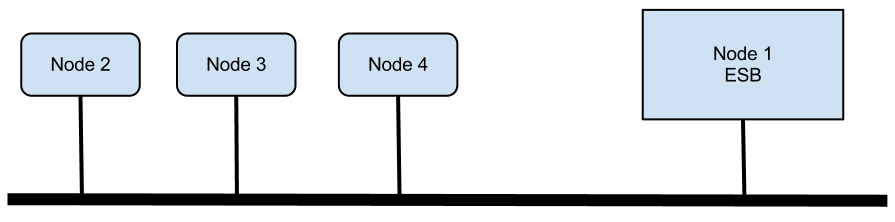
\includegraphics[width=\textwidth, scale=0.3]{NS3network}
        \caption{The layout of our network during testing}
        In this figure we have illustrated the layout of the network during NS3 testing.
        \label{fig:NS3network}
    \end{figure}
    
    This new layout limits the scope of the tests, and also what we could approve of functionality, but still we think we have a strong end product with results that will absolutely be relevant for the customer.
    
    The MobiEmu testing framework operates by creating \gls{LXC} and connecting these to tap bridges created by NS3. This then emulates any network possible to create in NS3. From the point of view of programs running inside the LXC, they are full Linux machines connected to a real network. This means that any program able to run on Linux should run properly inside the LXC and any messages they send out is sent through NS3. This means that we have full control over how our network behaves and we can emulate quite a lot of scenarios.
    
    When MobiEmu starts up it creates a number of LXCs, it then starts up NS3 outside of any LXC and connects each of the LXCs to a corresponding tap bridge in NS3. Inside each of the LXCs it then starts the experiment and waits for the whole thing to finish before it completes nicely. Before each run MobiEmu stores all files and folders in the whole folder in order to easily recreate an experiment. When the experiment is done the result files are moved into the result folder. \\
    
    Our tests are set up as follows. We have three clients, two clients with low priority and one client with high priority. They send messages to the ESB which is connected to the same LAN as all the clients. The specific test client we use is describe in the following section. In the section~\ref{Testing:Cases} we have a detailed description of the reason behind each case. We tested with several different bandwidths in order to test our setup and see how it handled a variety of different bandwidths. The last thing that we tested was using different "Timeout" values on the ESB, which was done in order to test what setting works better for the different bandwidths. We did it this way because of the static nature of configuration on the ESB, detailed in the section~\ref{Configuration of the ESB}.

 		\subsubsection{Test Client}\label{Testing:About:Client}
    In this section we will shortly describe the test client used for testing, "EchoClientClient.jar"(ref:~\ref{attachment:file:EchoClientClient jar}).

    The client starts by reading its configuration file. Its filename can be provided as the only command line argument, otherwise it defaults to "client.config'. This configuration file contains variables such as username, password, role, service to contact, what the request should be, how many requests to send and with what interval it should send them at, and some describing what to log.

    The client expects the request to contain '{REQID}' as part of the request message, and before sending it, the client will replace it with '{REQID=XX}' where 'XX' is the number of the request. This way the client can check that it gets the right response by checking whether '{REQID=XX}' is present in the response, and whether the ID is correct. This makes validating the response from the service easier, but it restricts the service to put the request message somewhere in the response. Another side effect of this being the only validation is that other errors in the response are not easily detected as long as the '{REQID=XX}' is there. If for example the response is cut short, by the stream being cut, as long as the ID is present it will be treated as valid. The client also prints the length of the response, so scripts that parse the results can pick up on responses with abnormal lengths.

    After reading the configuration file the client makes an instance of the client library described in section ~\ref{client side}, using the username, password and role, and itself as an ExceptionHandler. By implementing itself as the ExceptionHandler the client will be notified about all the exceptions occurring in the client library, the client does not act upon these exceptions, but it does log them. A normal client might want to send a request again here.
    
    A timer is used to start the sending/receiving in a new thread at the interval specified and the number of times specified. Starting new threads for every request and sending at a small interval is a good way to test how the client library handles concurrent requests.

    The actual sending and receiving of data is rather simple, as you can see in this code snippet:
    \lstset{language=Java, style=eclipse}
    \lstset{frame=single}
    \lstset{breaklines=true}
    \lstset{showstringspaces=false}
    \begin{lstlisting}
/* Uses connection.sendData(data, destination) to send a request. Here {REQID} in the request found in clientConfig is replaced with {REQID=reqID}. The client library will put the response in the returned ReceiveObject when it is received. */
ReceiveObject ro = connection.sendData(
config.get(DATA).replace("{"+REQID+"}", "{"+REQID+"="+reqID+"}"), destination);
try {
    logLine("Waiting for response "+reqID);

/* Calls the blocking method ReceiveObject.receive() to get the response. An alternative to this would be to make a DataListener and add it to connection This way, every listener would receive all the responses, and would be unsuited for this test */
    String response = ro.receive();
    \end{lstlisting}
    \\
    For more details about configuring the test client, read the example configuration provided in appendix ~\ref{attachment:file:Client config}. For more detailed information on how the test client works, the TestClient.java file with Javadoc is also provided in appendix ~\ref{attachment:file:TestClient java}.


    	\subsubsection{Test Service}\label{Testing:About:Service}
    In this section we will shortly describe the test service used for testing, \ref{attachment?}"EchoServiceLargeReply.war".
    % TODO: fix ref.

    The test service is very simple and deployable with GlassFish. It expects a request like this:
    \lstset{language=xml}
    \begin{lstlisting}
<?xml version="1.0" encoding="UTF-8"?>
<S:Envelope xmlns:S="http://schemas.xmlsoap.org/soap/envelope/">
    <S:Header/>
    <S:Body>
        <ns2:hello xmlns:ns2="http://me.test.org">
            <name>PAYLOAD</name>
        </ns2:hello>
    </S:Body>
</S:Envelope>
    \end{lstlisting}
    \\
    And responds like this:
    \begin{lstlisting}
<?xml version='1.0' encoding='utf-8'?>
<S:Envelope xmlns:S="http://schemas.xmlsoap.org/soap/envelope/">
    <S:Body>
        <ns2:helloResponse xmlns:ns2="http://me.test.org">
            <return>
                PAYLOAD!
                Lorem ipsum dolor sit amet, consectetur adipiscing elit. Etiam sodales magna at est iaculis vel fermentum velit tristique. Cras nulla urna, ultrices vitae posuere a, iaculis sit amet lectus. Aliquam mattis sapien et elit commodo ...
            </return>
        </ns2:helloResponse>
    </S:Body>
</S:Envelope>
    \end{lstlisting}
    \\
    With PAYLOAD intact, and 10KB of Lorem Ipsum\footnote{\url{http://www.lipsum.com/} - simply dummy text}. We add these 10KB of text to ensure that the response is considerably larger than the request, which should get us more realistic results when testing. We also send the original payload back so the test client can easily identify which request was responded to. Those 10KB of text also has a large impact on testing, it means that on lower than 10KBps bandwidth all the messages can't be sent in time. We chose to have it this way because it would give us a predictable test and also some static configuration on the ESB could be configured with this in mind.

    	\subsubsection{Strengths And Weaknesses}\label{Testing:About:Strengths}
	There are some weaknesses connected with our testing suite and how we do the testing. Chief among them is the limited scope made necessary by limitations encountered in NS3. However there are other areas where the testing suite could be expanded which could be done without butting heads with NS3.
	
	One limitation that was self imposed is the fact that we only have one test network layout. This should have been expanded, but because of limited time at the end of the project we chose to focus more on the one test. With a more expanded network layout, which is quite feasible despite the problems encountered with NS3, one could add more clients and introduce several priorities to test how the ESB would behave. We theorize that the ESB should behave in the same way and we have created it in such a way to prioritize the highest priority messages no matter what the other messages does.
	
	Another limitation to the test setup is that we have no easy way to communicate between the LXCs. What this means is that we can not coordinate when to terminate the whole test. What this means is that we have to enforce a cutoff time which does skew some test. Especially bad is this when we run the test without our Throttle mediator. Because without our Throttle mediator even on the lower bandwidths no messages should be lost and the percentage of successful messages should be one. This will effect the test, but we decided to keep it this way because we mean the general trend on the results are still clear.
	
	The test client also has some problems. For one it does not try to retransmit any messages. This has a profound effect on the results regarding successful message percentage which will be quite different with and without our Throttle mediator. With our Throttle mediator we will perceive a lower percentage compared to without the mediator, but this is just a result of us dropping messages which retransmitting would to some degree correct.

	\subsection{Test Cases}\label{Testing:Cases}
			\subsection{Test Cases}\label{Testing:Cases}

	As most of the tests below are quite alike the reasoning behind them are also quite like. The main difference between them are the “Timeout” which refer to the timeout the ESB uses. For more about the “Timeout” see \ref{Configuration of the ESB}.

	Since this project had somewhat of a research focus from the customers side we did not perform these test in order for us to validate our system. Instead we have run these tests to try and say something about the feasibility of the original question asked when we started. We will come back to this topic in the result section.\\
    
    We used the same client setups for all of the tests. The low priority clients, Client 1 and 2, was configured like this:
\lstset{language=matlab}
\begin{lstlisting}
%This is a comment
%variables are written with NAME:VALUE
%line without ':' or '%' is treated as end of file.
%doLog:boolean, whether to log or not, default is true.
doLog:true
%logToFile:boolean, whether or not client library should log to file, default is false.
logToFile:true
%username:String, Must be configured.
username:testname
%password:String, Must be configured.
password:testpassword
%role:String, Must be configured.
role:clientRole1
%service:URI, Must be configured.
service:https://10.0.0.1:8243/services/EchoService
%interval:long, between requests in milliseconds, only one request if not configured
interval:1000
%nofreqs: int, number of requests to send, send forever if not configured
nofreqs:100
%delay:long, wait before first request in milliseconds, default is 0
delay:10
%request:SOAP, Must be configured.
request:<?xml version="1.0" encoding="UTF-8"?><S:Envelope xmlns:S="http://schemas.xmlsoap.org/soap/envelope/"><S:Header/><S:Body><ns2:hello xmlns:ns2="http://me.test.org"><name>{REQID}</name></ns2:hello></S:Body></S:Envelope>
\end{lstlisting}
    Client 2 had 0 as delay. While the high priority client, Client 3, had interval=3000, nofreqs=30 and delay=15.
\begin{center}

\begin{tabular}{| p{4cm} | p{8cm} |}%\label{test:1}
	\hline
	ID & 1 \\
	\hline
	Description &  In this test what we are looking at is how our system behaves with a very low timeout, since we have full control over the message sizes sent in the test we know that this timeout will be too low on the lower bandwidths, but should perform much better on high bandwidths. \\
	\hline
	Repetition(s) & 10 \\
	\hline
	NS3 variables & Datarate: 1kBps,5kBps,10kBps,20kBps,40kBps \\
	\hline
	ESB variables & \textbf{Timeout: 500}, interval: 500, minimum bandwidth per message: 10240 \\
	\hline
	Automated & Yes \\
	\hline
	Expected Result & We expect to see that the ESB will time out even higher priority messages in the lower bandwidth tests because of the low timeout, but on higher bandwidths the sending time of the all the messages should be lower than on the later tests. To put that in the same setting as our results, we expect the percentage of successfully received messages to be lower than in the tests below, but we expect the time to also be lower across the board.  \\
	\hline
	Folder with compressed test & In appendix \ref{attachment:file:Test Case 1} you can find the appropriate compressed test case.\\
	\hline
\end{tabular}

\\ \ldots \\

\begin{tabular}{| p{4cm} | p{8cm} |}%\label{test:2}
	\hline
	ID & 2 \\
	\hline
	Description & In this test we have increased the timeout substantially, we expect to see some improvements on 10kBps and still retain some of the benefits of a lower timeout on 20- and 40kBps \\
	\hline
	Repetition(s) & 10 \\
	\hline
	NS3 variables & Datarate: 1kBps,5kBps,10kBps,20kBps,40kBps \\
	\hline
	ESB variables & \textbf{Timeout: 1000}, interval: 500, minimum bandwidth per message: 10240 \\
	\hline
	Automated & Yes \\
	\hline
	Expected Result & We expect to have a higher percentage of completed messages on 10kBps than with a timeout of 500 and we expect the results on 1-, 20- and 40kBps to be relatively unchanged. \\
	\hline
	Folder with compressed test & In appendix \ref{attachment:file:Test Case 2} you can find the appropriate compressed test case.\\
	\hline
\end{tabular}

\\ \ldots \\

\begin{tabular}{| p{4cm} | p{8cm} |}%\label{test:3}
	\hline
	ID & 3 \\
	\hline
	Description & Again we have increased the timeout and expect to see some improvements on percentage, but we the total time taken should start to drop on higher bandwidths.  \\
	\hline
	Repetition(s) & 10 \\
	\hline
	NS3 variables & Datarate: 1kBps,5kBps,10kBps,20kBps,40kBps \\
	\hline
	ESB variables & \textbf{Timeout: 2000}, interval: 500, minimum bandwidth per message: 10240 \\
	\hline
	Automated & Yes \\
	\hline
	Expected Result & We expect all the messages on 20 and 40kBps to arrive, we expect that on 10kBps more messages should arrive, but not all. The time taken should again increase. \\
	\hline
	Folder with compressed test & In appendix \ref{attachment:file:Test Case 3} you can find the appropriate compressed test case.\\
	\hline
\end{tabular}

\\ \ldots \\

\begin{tabular}{| p{4cm} | p{8cm} |}%\label{test:4}
	\hline
	ID & 4 \\
	\hline
	Description & In this test we want to see how the ESB copes with a much larger timeout.  \\
	\hline
	Repetition(s) & 10 \\
	\hline
	NS3 variables & Datarate: 1kBps,5kBps,10kBps,20kBps,40kBps \\
	\hline
	ESB variables & \textbf{Timeout: 5000}, interval: 500, minimum bandwidth per message: 10240 \\
	\hline
	Automated & Yes \\
	\hline
	Expected Result & We expect that 10-, 20- and 40kBps should be enough to get most of the messages for the high priority client through, the time taken should again increase and this should be noticeable on 40kBps compared to Test 1.  \\
	\hline
	Folder with compressed test & In appendix \ref{attachment:file:Test Case 4} you can find the appropriate compressed test case.\\
	\hline
\end{tabular}

\\ \ldots \\

\begin{tabular}{| p{4cm} | p{8cm} |}%\label{test:5}
	\hline
	ID & 5 \\
	\hline
	Description & In this test we have gone all out. The timeout is massivly increased to see how the ESB behaves on the lowest bandwidths, 1- and 5kBps respectively.  \\
	\hline
	Repetition(s) & 10 \\
	\hline
	NS3 variables & Datarate: 1kBps,5kBps,10kBps,20kBps,40kBps \\
	\hline
	ESB variables & \textbf{Timeout: 100 000}, interval: 500, minimum bandwidth per message: 10240 \\
	\hline
	Automated & Yes \\
	\hline
	Expected Result & We expect the same percentage on 10-, 20- and 40kBps as Test 4. What we want to see is that on 5kBps the percentage is increased quite substantially compared to the previous tests. \\
	\hline
	Folder with compressed test & In appendix \ref{attachment:file:Test Case 5} you can find the appropriate compressed test case.\\
	\hline
\end{tabular}
\\ \ldots \\
\begin{tabular}{| p{4cm} | p{8cm} |}%\label{test:6}
	\hline
	ID & 6 \\
	\hline
	Description & In this test what we have done is to remove our Throttle mediator which should mean that our ESB setup will no longer be doing any throttling of messages. The message queue is still there so there will be some priority in the sending and receiving. We want to test this because this should give us some idea about how our setup will do against no QoS at all. \\
	\hline
	Repetition(s) & 10 \\
	\hline
	NS3 variables & Datarate: 1kBps,5kBps,10kBps,20kBps,40kBps \\
	\hline
	ESB variables & \textbf{Timeout: N/A}, interval: 500, minimum bandwidth per message: N/A \\
	\hline
	Automated & Yes \\
	\hline
	Expected Result & We expect that the average percentage of all the clients will be slightly above what our test can do, we refer to section \ref{Testing:About:Weaknesses} for some elaboration about this. What we want to see is that on lower bandwidths the average time taken for messages to arrive at Client 4 will be substantially higher than when we use the Throttle mediator. This will indicate that our Throttle mediator actually does some useful work and also indicate that this could be a viable strategy for our customer to continue researching. \\
	\hline
	Folder with compressed test & In appendix \ref{attachment:file:Test Case 6} you can find the appropriate compressed test case. \\
	\hline
\end{tabular}

\\ \ldots \\

\end{center}

	\subsection{Results}\label{Testing:Results}
		[Here be results]
    % test results.
